%%\documentclass[a4paper,12pt,oneside]{llncs}
\documentclass[12pt,letterpaper]{article}
\usepackage[right=2cm,left=3cm,top=2cm,bottom=2cm,headsep=0cm]{geometry}

%%%%%%%%%%%%%%%%%%%%%%%%%%%%%%%%%%%%%%%%%%%%%%%%%%%%%%%%%%%
%% Juego de caracteres usado en el archivo fuente: UTF-8
\usepackage{ucs}
\usepackage[utf8x]{inputenc}

%%%%%%%%%%%%%%%%%%%%%%%%%%%%%%%%%%%%%%%%%%%%%%%%%%%%%%%%%%%
%% Juego de caracteres usado en la salida dvi
%% Otra posibilidad: \usepackage{t1enc}
\usepackage[T1]{fontenc}

%%%%%%%%%%%%%%%%%%%%%%%%%%%%%%%%%%%%%%%%%%%%%%%%%%%%%%%%%%%
%% Ajusta maergenes para a4
%\usepackage{a4wide}

%%%%%%%%%%%%%%%%%%%%%%%%%%%%%%%%%%%%%%%%%%%%%%%%%%%%%%%%%%%
%% Uso fuente postscript times, para que los ps y pdf queden y pequeños...
\usepackage{times}

%%%%%%%%%%%%%%%%%%%%%%%%%%%%%%%%%%%%%%%%%%%%%%%%%%%%%%%%%%%
%% Posibilidad de hipertexto (especialmente en pdf)
%\usepackage{hyperref}
\usepackage[bookmarks = true, colorlinks=true, linkcolor = black, citecolor = black, menucolor = black, urlcolor = black]{hyperref}

%%%%%%%%%%%%%%%%%%%%%%%%%%%%%%%%%%%%%%%%%%%%%%%%%%%%%%%%%%%
%% Graficos 
\usepackage{graphics,graphicx}

%%%%%%%%%%%%%%%%%%%%%%%%%%%%%%%%%%%%%%%%%%%%%%%%%%%%%%%%%%%
%% Ciertos caracteres "raros"...
\usepackage{latexsym}

%%%%%%%%%%%%%%%%%%%%%%%%%%%%%%%%%%%%%%%%%%%%%%%%%%%%%%%%%%%
%% Matematicas aun más fuertes (american math dociety)
\usepackage{amsmath}

%%%%%%%%%%%%%%%%%%%%%%%%%%%%%%%%%%%%%%%%%%%%%%%%%%%%%%%%%%%
\usepackage{multirow} % para las tablas
\usepackage[spanish,es-tabla]{babel}

%%%%%%%%%%%%%%%%%%%%%%%%%%%%%%%%%%%%%%%%%%%%%%%%%%%%%%%%%%%
%% Fuentes matematicas lo mas compatibles posibles con postscript (times)
%% (Esto no funciona para todos los simbolos pero reduce mucho el tamaño del
%% pdf si hay muchas matamaticas....
\usepackage{mathptm}

%%% VARIOS:
\usepackage{slashbox}
\usepackage{verbatim}
\usepackage{array}
\usepackage{listings}
\usepackage{multirow}

%% MARCA DE AGUA
%% Este package de "draft copy" NO funciona con pdflatex
%%\usepackage{draftcopy}
%% Este package de "draft copy" SI funciona con pdflatex
%%%\usepackage{pdfdraftcopy}
%%%%%%%%%%%%%%%%%%%%%%%%%%%%%%%%%%%%%%%%%%%%%%%%%%%%%%%%%%%
%% Indenteacion en español...
\usepackage[spanish]{babel}

\usepackage{listings}
% Para escribir código en C
% \begin{lstlisting}[language=C]
% #include <stdio.h>
% int main(int argc, char* argv[]) {
% puts("Hola mundo!");
% }
% \end{lstlisting}


\title{Análisis}
\author{Jesús Rodríguez Heras}

\begin{document}
	
	\maketitle
	\begin{abstract} %Poner esto en todas las prácticas de PCTR
		\begin{center}
			Análisis de resultados del ejercicio 3 de la práctica 12.
		\end{center}
	\end{abstract}
	\thispagestyle{empty}
	\newpage
	
%	\tableofcontents
%	\newpage
	
	%%\listoftables
	%%\newpage
	
	%%\listoffigures
	%%\newpage
	
	%%%% REAL WORK BEGINS HERE:
	
	%%Configuracion del paquete listings
	\lstset{language=bash, numbers=left, numberstyle=\tiny, numbersep=10pt, firstnumber=1, stepnumber=1, basicstyle=\small\ttfamily, tabsize=1, extendedchars=true, inputencoding=latin1}

\section{Tiempos para el ejercicio 3}
\section{Tiempos para el ejercicio 1}
\subsection{Windows}
\begin{center}
	\begin{table}[htbp]
		\begin{center}
			\begin{tabular}{|c|c|c|}
				\hline
				& \multicolumn{1}{c|}{C++} & \multicolumn{1}{c|}{Java}  \\
				\hline
				Vueltas  & pcHebras & pcHebras \\\hline
				1000 & 0.415 & 0.032  \\\hline
				2000 & 0.937 & 0.031  \\\hline
				3000 & 1.2 & 0.053  \\\hline
				4000 & 1.584 & 0.051  \\\hline
				5000 & 2.073 & 0.047  \\\hline
				6000 & 2.419 & 0.062  \\\hline
				7000 & 2.784 & 0.063  \\\hline
				8000 & 3.23 & 0.069  \\\hline
				9000 & 3.617 & 0.068  \\\hline
				10000 & 3.953 & 0.084  \\\hline
			\end{tabular}
			\caption{Valores en segundos del tiempo usado por cada algoritmo.}
			\label{tabla:Valores en segundos del tiempo usado por cada algoritmo}
		\end{center}
	\end{table}
\end{center}


\subsection{Linux}
\begin{center}
	\begin{table}[htbp]
		\begin{center}
			\begin{tabular}{|c|c|c|}
				\hline
				& \multicolumn{1}{c|}{C++} & \multicolumn{1}{c|}{Java}  \\
				\hline
				Vueltas  & pcHebras & pcHebras \\\hline
				1000 & 0.009 & 0.034  \\\hline
				2000 & 0.011 & 0.053  \\\hline
				3000 & 0.015 & 0.067  \\\hline
				4000 & 0.017 & 0.057  \\\hline
				5000 & 0.021 & 0.063  \\\hline
				6000 & 0.026 & 0.068  \\\hline
				7000 & 0.036 & 0.07  \\\hline
				8000 & 0.034 & 0.071  \\\hline
				9000 & 0.034 & 0.066  \\\hline
				10000 & 0.034 & 0.078  \\\hline
			\end{tabular}
			\caption{Valores en segundos del tiempo empleado por cada algoritmo.}
			\label{tabla:Valores en segundos del tiempo empleado cada algoritmo}
		\end{center}
	\end{table}
\end{center}
\section{Gráficas}
\newpage

\begin{center}
	\begin{figure}
		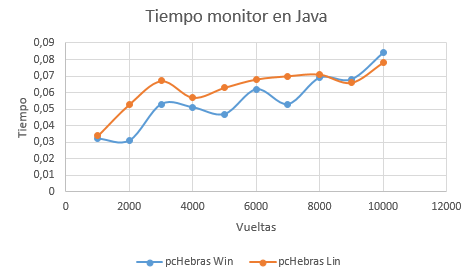
\includegraphics[scale=1.3]{TiempoMonitorJava.png}
	\end{figure}
\end{center}

\begin{center}
	\begin{figure}
		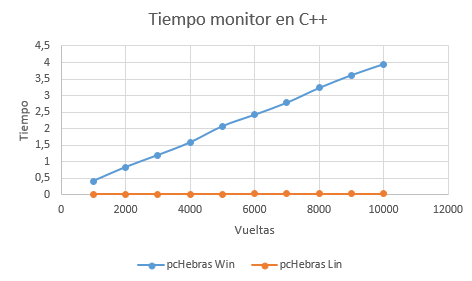
\includegraphics[scale=1.3]{TiempoMonitorC.png}
	\end{figure}
\end{center}





\end{document}